\documentclass[aspectratio=169]{beamer}

\usepackage[utf8]{inputenc}
%\usepackage{emoji}

\usepackage{amsmath}
\usepackage{graphicx}
\usepackage[T1]{fontenc}
\usepackage{libertine}
\usepackage{array}
\usepackage{marvosym}
\usepackage{bm}

\usepackage{pgfplots}
\usepackage{tikz}
\usetikzlibrary{automata, arrows, positioning, calc, external, babel, backgrounds, matrix, shapes, shadings}
\usepgfplotslibrary{fillbetween}


%%natbib conf
\usepackage[square,authoryear]{natbib}
\renewcommand{\cite}{\citep}
\renewcommand{\bibfont}{\small}
\bibliographystyle{abbrvnat} 

\newcommand{\R}{\mathbb{R}}
\newcommand{\brackets}[2]{\left\langle#1,#2\right\rangle}
\newcommand{\ind}[1]{\mathbf{1}_{\left\{#1\right\}}}

\newcommand{\graphheight}{7cm}
\newcommand{\graphwidth}{11cm}

\newcommand{\E}[1]{E\left[#1 \right]}
\renewcommand{\phi}{\varphi}

% \definecolor{azulcito}{RGB}{20,70,140}
\definecolor{azulcito}{RGB}{0,90,150}
\definecolor{verdecito}{RGB}{90,150,0}
\definecolor{rojito}{RGB}{150,0,90}
\definecolor{violetita}{RGB}{150,20,150}


\setbeamercolor*{structure}{fg=azulcito,bg=azulcito!20!white}
\setbeamercolor*{alerted text}{fg=azulcito}

  \setbeamercolor{block title}{fg=azulcito,bg=azulcito!20!white}
  \setbeamercolor{block body}{fg=black,bg=azulcito!10!white}
  
\beamertemplatenavigationsymbolsempty

\setbeamercolor*{author in head/foot}{fg=azulcito,bg=azulcito!15!white}
\setbeamercolor*{title in head/foot}{fg=azulcito,bg=azulcito!15!white}
\setbeamercolor*{date in head/foot}{fg=azulcito,bg=azulcito!15!white}

% Pgfplots
\pgfplotsset{width=\graphwidth, height = \graphheight, grid style = {dashed, gray}, every tick label/.append style = {font=\footnotesize}, compat=1.18, legend style={font=\footnotesize, draw=none, fill=none}, every axis/.append style={label style={font=\footnotesize}}}

\tikzset{>=stealth}

\newtheorem{proposition}{Proposition}
%\newtheorem{definition}{Definition}
%\newtheorem{lemma}{Lemma}
%\newtheorem{corollary}{Corollary}

\defbeamertemplate*{footline}{mitema}
{
  \leavevmode%
  \hbox{%
  \begin{beamercolorbox}[wd=.25\paperwidth,ht=2.25ex,dp=1ex,left]{author in head/foot}%
    \usebeamerfont{author in head/foot}\hspace*{2ex}\insertshortauthor
  \end{beamercolorbox}%
  \begin{beamercolorbox}[wd=.5\paperwidth,ht=2.25ex,dp=1ex,center]{title in head/foot}%
    \usebeamerfont{date in head/foot}\insertshortdate{}
  \end{beamercolorbox}%
  \begin{beamercolorbox}[wd=.25\paperwidth,ht=2.25ex,dp=1ex,right]{date in head/foot}%
    \insertframenumber{}/\inserttotalframenumber\hspace*{2em} 
  \end{beamercolorbox}}%
 \vskip0pt%
}


\setbeamercolor{blocky}{fg=azulcito,bg=azulcito!15!white}
\setbeamercolor{blocky2}{fg=black,bg=azulcito!10!white}

\defbeamertemplate*{title page}{customized}[1][]
{
{\flushright
  \begin{beamercolorbox}[wd=\paperwidth,sep=1em,right,rightskip=1.5em]{blocky}%
    \usebeamerfont{title}{\huge \inserttitle}\par \bigskip

    \usebeamerfont{subtitle}{\large \insertsubtitle}\par
  \end{beamercolorbox}%
  \vfill
    \usebeamerfont{author}{\Large \insertauthor}\par \vspace{1em}
      \usebeamerfont{institute}{\large \insertinstitute}\par
  
  
  \vfill
  \usebeamerfont{date}{\insertdate}\par
  %\usebeamercolor[fg]{titlegraphic}\inserttitlegraphic
  }
}

\usefonttheme[onlymath]{serif}

% ============================================================
\title[PDMPs: Theory \& Stationary Distributions]{
  Piecewise-Deterministic Markov Processes}
\subtitle{Theory and Methods for Stationary Distributions}
\author[A. Ferragut]{Andres Ferragut}
\date{Universidad ORT Uruguay}

\begin{document}

% ============================================================
\begin{frame}
  \titlepage
\end{frame}

% ============================================================
\begin{frame}{Outline}
  \tableofcontents
\end{frame}

% ============================================================
\section{Motivation and Context}

 \begin{frame}{Piecewise deterministic Markov processes}
   \begin{columns}
     \begin{column}{0.55\textwidth}
       Davis (1984) observed that continuous-time stochastic models consist of:
       \begin{enumerate}
         \item \textbf{Diffusion} (Brownian noise)
         \item \textbf{Deterministic motion}
         \item \textbf{Random jumps}
       \end{enumerate}
       \bigskip
       \begin{block}{The Gap}
         Diffusion theory is highly unified (It\^o calculus).
         Non-diffusion models~--- ingredients (2)+(3)~--- were a
         \emph{heterogeneous collection of special cases}.
       \end{block}
     \end{column}
    \begin{column}{0.42\textwidth}
      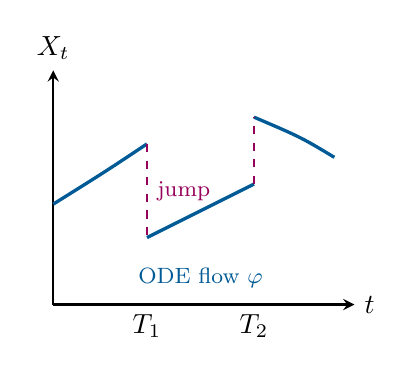
\begin{tikzpicture}[scale=0.85]
        \draw[->,thick] (0,0) -- (4.5,0) node[right]{$t$};
        \draw[->,thick] (0,0) -- (0,3.5) node[above]{$X_t$};
        % ODE segments
        \draw[azulcito,very thick] (0,1.5) .. controls (0.8,2.0) .. (1.4,2.4);
        \draw[azulcito,very thick] (1.4,1.0) .. controls (2.2,1.4) .. (3.0,1.8);
        \draw[azulcito,very thick] (3.0,2.8) .. controls (3.7,2.5) .. (4.2,2.2);
        % Jumps
        \draw[rojito,dashed,thick] (1.4,2.4) -- (1.4,1.0)
          node[midway,right]{\footnotesize jump};
        \draw[rojito,dashed,thick] (3.0,1.8) -- (3.0,2.8);
        \node[below] at (1.4,0) {$T_1$};
        \node[below] at (3.0,0) {$T_2$};
        \node[azulcito] at (2.2,0.4) {\footnotesize ODE flow $\phi$};
      \end{tikzpicture}
    \end{column}
  \end{columns}
  \bigskip
  \pause
  \alert{Goal:} Provide a \emph{canonical class} covering virtually all non-diffusion models,
  with a unified stochastic calculus analogous to diffusion theory.
 \end{frame}

% ============================================================
\begin{frame}{Motivating Examples}
  \begin{columns}[T]
    \begin{column}{0.48\textwidth}
      \textbf{Classical examples (Davis 1984)}
      \begin{itemize}
        \item Countable-state Markov processes
        \item Non-exponential sojourn-time processes
        \item $M/G/1$ and $GI/G/1$ queues (virtual waiting time)
        \item Dam / storage / release models
      \end{itemize}
    \end{column}
    \begin{column}{0.48\textwidth}
      \textbf{Modern applications}
      \begin{itemize}
        \item TCP/IP congestion control
        \item Reliability \& maintenance models
        \item Biochemical reaction networks
        \item Risk / ruin theory (insurance)
      \end{itemize}
    \end{column}
  \end{columns}
  \bigskip
  \begin{alertblock}{Key claim (Davis 1984)}
    The class is \emph{``wide enough to include as special cases virtually all the
    non-diffusion models of applied probability.''}
  \end{alertblock}
\end{frame}

% ============================================================
\section{Definition of the PDMP}

\begin{frame}{Local Characteristics}
  A PDMP on $E \subseteq \R^d$ (open) is determined by three objects:

  \vfill

  \only<1>{
      \begin{block}{(1) The flow $\phi$}
        Unique solution map of
        $\dot{x} = f(x)$, so
        \[
          \phi(0,x)=x
        \]
        \[
          \phi(t{+}s,x)=\phi(t,\phi(s,x))
        \]
        Assumes $f$ is Lipschitz continuous.
      \end{block}
  }
  \only<2>{
    
      \begin{block}{(2) The jump rate function $\lambda$}
        Measurable $\lambda:E\to\R_+$.\\[4pt]
        Integrated rate:
        \[
          \Lambda(t,x)=\int_0^t \!\lambda(\phi(s,x))\,\mathrm{d} s
        \]
        governs the Poisson-like clock.
      \end{block}
  }
  \only<3>{
      \begin{block}{(3) The jump kernel $Q$}
        Probability measure $Q(x,\cdot)$ on $E$.\\[4pt]
        Post-jump location
        \[
          Z_1 \sim Q(\phi(T_1,x_0),\cdot)
        \]
        drawn independently of $T_1$.
      \end{block}
    }
	\vfill
\end{frame}

% ============================================================
\begin{frame}{The Integrated Hazard Rate $\Lambda$}
 
  The function $\lambda : E \to \mathbb{R}_+$ is a \textbf{hazard rate}: it measures
  the instantaneous intensity of jumping \emph{at the current location of the flow}.
 
  \bigskip
  Because the process moves deterministically between jumps, the relevant
  object is the \textbf{integrated hazard along the trajectory}:
  \[
    \Lambda(t,x) \;=\; \int_0^t \lambda\!\bigl(\phi(s,x)\bigr)\,\mathrm{d}s.
  \]
  This is the cumulative intensity seen by a particle starting at $x$ and
  following the ODE flow for time $t$.
 
  \bigskip
  The first jump time $T_1$ is then defined as a \emph{non-homogeneous
  exponential} with this integrated rate:
  \[
    P(T_1 > t \mid X_0 = x) \;=\; e^{-\Lambda(t,\,x)}.
  \]
 
  \bigskip
 
\end{frame}
 
\begin{frame}{Boundary condition}

\begin{itemize}
  \item \textbf{Reachable boundary:} $\partial^* E = \{z \in \partial E : \phi(-t,z) \in E
        \text{ for all } t \in (0,\varepsilon),\ \text{some } \varepsilon > 0\}$ —
        boundary points that the flow can reach from inside $E$.
  \item \textbf{Boundary exit time:}
        $t^*(x) = \inf\{t > 0 : \phi(t,x) \in \partial^* E\}$,
        with $t^*(x) = \infty$ if the flow never reaches $\partial^* E$.
\end{itemize}

\vfill
  \begin{alertblock}{Davis's Assumption (boundary jumps)}
    If the flow reaches the boundary in finite time, i.e.\ $t^*(x) < \infty$,
    Davis assumes
    \[
      \Lambda(t^*(x),\,x) = \infty.
    \]
    Consequence: $P(T_1 < t^*(x)) = 1$, so the Poisson clock \emph{always fires
    before the boundary is reached}.  Forced boundary jumps are excluded.
  \end{alertblock}

  \vfill

  \alert{Remark:} Costa (1990) relaxes this assumption.
\end{frame}

% --- Slide B: The actual construction, cleaned up ----------------------------
\begin{frame}{Sample Path Construction}
 
  Starting from $x_0 \in E$, one inter-jump cycle is constructed as follows.
 
  \bigskip
  \begin{enumerate}
    \setlength\itemsep{8pt}
 
    \item \textbf{Draw the alarm level.}
          Sample $U \sim \mathrm{Uniform}(0,1)$ and set $s^* = -\log U > 0$.
 
    \item \textbf{Run the flow and clock jointly.}
          Integrate $\dot{x} = f(x)$ from $x_0$ while simultaneously
          accumulating $\Lambda(t,x_0) = \int_0^t \lambda(\phi(s,x_0))\,\mathrm{d}s$.
          Stop at the first time
          \[
            T_1 = \inf\bigl\{t > 0 : \Lambda(t,x_0) \geq s^*\bigr\}.
          \]
          Under Davis's assumption, $T_1 < t^*(x_0)$ with probability~$1$.
 
    \item \textbf{Draw the post-jump location.}
          Sample $Z_1 \sim Q\left(\phi(T_1,x_0),\,\cdot\,\right)$
          independently of $T_1$.
 
    \item \textbf{Restart.}
          Set $X_{T_1} = Z_1$ and repeat from step~1.
  \end{enumerate}
  
\end{frame}

\begin{frame}{Markov Property and Non-Explosion}

  \begin{block}{Markov property}
    The semigroup property of $\varphi$ ensures the process is
    \textbf{strong Markov}: the distribution of the next jump time
    depends only on the current state $X_t$, not on the history.
  \end{block}

  \bigskip
  \begin{block}{Non-explosion (Davis, Assumption~3.1)}
    Require $E[N_t] < \infty$ for all $t \geq 0$, equivalently
    $T_n \to \infty$ a.s., so the process does not accumulate
    infinitely many jumps in finite time.
  \end{block}

  \bigskip
  \begin{alertblock}{Remark}
    Non-explosion is not automatic --- it must be verified for each
    model. For the TCP/IP example, it follows from Foster's criterion
    applied later.
  \end{alertblock}

\end{frame}

\begin{frame}{Example: TCP/IP Congestion Control}

  \begin{block}{Informal description}
    A TCP flow increases its sending rate continuously (deterministic motion)
    and suffers random packet loss events (jumps) that halve the rate
    --- the classical AIMD mechanism.
  \end{block}

  \vfill
  \textbf{Local characteristics:}
  \begin{itemize}
    \setlength\itemsep{6pt}
    \item \textbf{State space:} $E = \mathbb{R}_+$, where $x$ is the current
          sending rate.

    \item \textbf{Flow:} $f(x) = c > 0$ (additive increase), so
          $\phi(t,x) = x + ct$.

    \item \textbf{Jump rate:} $\lambda(x) = \alpha x$, $\alpha > 0$ ---
          loss probability grows with the sending rate.

    \item \textbf{Jump kernel:} $Q(x,\,\cdot\,) = \delta_{x/2}$ ---
          upon a loss event the rate is halved.
  \end{itemize}
  \vfill
\end{frame}

\begin{frame}{Example: TCP/IP Congestion Control}
  
  \vfill

  \begin{center}
    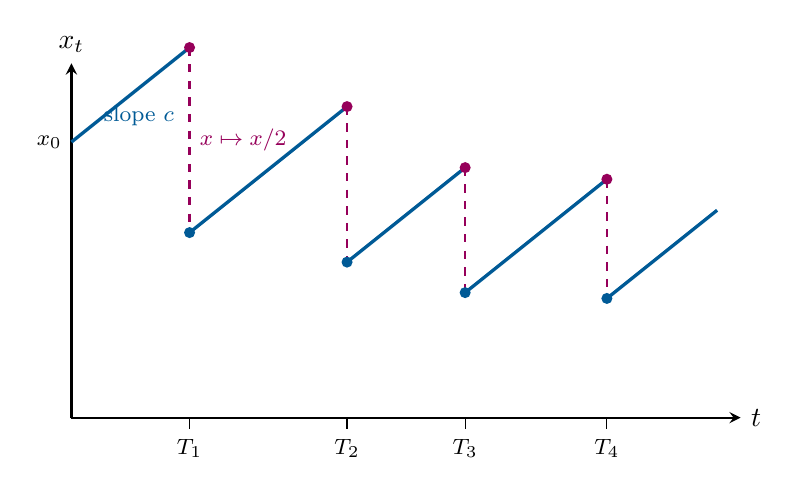
\begin{tikzpicture}
        % Axes
        \draw[->,thick] (0,0) -- (8.5,0) node[right]{$t$};
        \draw[->,thick] (0,0) -- (0,4.5) node[above]{$x_t$};

        % Segment 0: start at x0=3.5, slope c, until T1
        % T1 at t=1.5, x=3.5+1.5*0.8=4.7 -> jump to 4.7/2=2.35
        \draw[azulcito,very thick] (0,3.5) -- (1.5,4.7) node[midway,below, xshift=+3pt] {\footnotesize slope $c$};
        \draw[rojito,dashed,thick]  (1.5,4.7) -- (1.5,2.35) node[midway, right,font=\footnotesize]{$x \mapsto x/2$};
        \fill[rojito] (1.5,4.7)  circle (2pt);
        \fill[azulcito] (1.5,2.35) circle (2pt);

        % Segment 1: start at 2.35, slope c, until T2
        % T2 at t=3.5, x=2.35+2*0.8=3.95 -> jump to 3.95/2=1.975
        \draw[azulcito,very thick] (1.5,2.35) -- (3.5,3.95);
        \draw[rojito,dashed,thick]  (3.5,3.95) -- (3.5,1.975);
        \fill[rojito] (3.5,3.95)  circle (2pt);
        \fill[azulcito] (3.5,1.975) circle (2pt);

        % Segment 2: start at 1.975, slope c, until T3
        % T3 at t=5.0, x=1.975+1.5*0.8=3.175 -> jump to 3.175/2=1.5875
        \draw[azulcito,very thick] (3.5,1.975) -- (5.0,3.175);
        \draw[rojito,dashed,thick]  (5.0,3.175) -- (5.0,1.5875);
        \fill[rojito] (5.0,3.175)  circle (2pt);
        \fill[azulcito] (5.0,1.5875) circle (2pt);

        % Segment 3: start at 1.5875, slope c, until T4
        % T4 at t=6.8, x=1.5875+1.8*0.8=3.0275 -> jump to 3.0275/2=1.51375
        \draw[azulcito,very thick] (5.0,1.5875) -- (6.8,3.0275);
        \draw[rojito,dashed,thick]  (6.8,3.0275) -- (6.8,1.51375);
        \fill[rojito] (6.8,3.0275)  circle (2pt);
        \fill[azulcito] (6.8,1.51375) circle (2pt);

        % Segment 4: start at 1.51375, slope c, to end
        \draw[azulcito,very thick] (6.8,1.51375) -- (8.2,2.63375);

        % Jump times on x axis
        \foreach \t/\name in {1.5/$T_1$, 3.5/$T_2$, 5.0/$T_3$, 6.8/$T_4$}{
          \draw[thin] (\t,0) -- (\t,-0.15) node[below,font=\footnotesize]{\name};
        }

        % x0 label
        \node[left,font=\footnotesize] at (0,3.5) {$x_0$};
      \end{tikzpicture}
  \end{center}

  \vfill

\end{frame}



% ============================================================
% ============================================================
% Slide 1: Motivation
% ============================================================
\begin{frame}{The Generator: Motivation}

  We want to characterize how $E[\psi(X_t)]$ evolves. For a smooth test
  function $\psi: E \to \mathbb{R}$, track $\psi(X_t)$ along a sample path.

  \bigskip
  \textbf{Between jumps:} $X_t = \varphi(t,x)$ follows the ODE, so by the
  chain rule:
  \[
    \frac{d}{dt}\psi(\varphi(t,x)) = f(\varphi(t,x))\cdot\nabla\psi(\varphi(t,x)).
  \]
  The instantaneous rate of change is the \textbf{directional derivative of
  $\psi$ along the vector field $f$}.

  \bigskip
  \textbf{At a jump time $T_i$:} the process jumps from $X_{T_i^-}$ to
  $Z_i \sim Q(X_{T_i^-}, \cdot)$, so $\psi$ changes by:
  \[
    \psi(Z_i) - \psi(X_{T_i^-}).
  \]
  Taking expectations, the average jump contribution at $x$ is:
  \[
    \lambda(x)\int_E [\psi(y) - \psi(x)]\,Q(x,\mathrm{d}y).
  \]

  \bigskip
  \begin{block}{Combining both effects}
    The generator $\mathcal{A}$ should capture the deterministic drift
    \emph{and} the average effect of jumps:
    \[
      \mathcal{A}\psi(x) = f(x)\cdot\nabla\psi(x)
      + \lambda(x)\int_E[\psi(y)-\psi(x)]\,Q(x,\mathrm{d}y).
    \]
  \end{block}

\end{frame}

% ============================================================
% Slide 2: Domain conditions
% ============================================================
\begin{frame}{The Generator: Domain $\mathcal{D}(\mathcal{A})$}

  Not every function $\psi$ can be in the domain of $\mathcal{A}$. Davis
  identifies three conditions.

  \bigskip
  \begin{enumerate}
    \setlength\itemsep{10pt}

    \item \textbf{Absolute continuity along trajectories.}
          $t \mapsto \psi(\varphi(t,x))$ is absolutely continuous on
          $[0,t^*(x))$ for each $x \in E$.\\
          \textit{Why:} ensures the directional derivative
          $f(x)\cdot\nabla\psi(x)$ exists Lebesgue-a.e.\ along each
          trajectory, so the ODE contribution is well defined.

    \item \textbf{Boundary condition.}
          $\psi(x) = \int_E \psi(y)\,Q(x,\mathrm{d}y)$ for all
          $x \in \partial^* E$.\\
          \textit{Why:} relevant when Davis's assumption is relaxed and
          forced boundary jumps can occur (Costa 1990). Under Davis's
          assumption this condition is vacuous.

    \item \textbf{Integrability.}
          $\mathcal{B}\psi \in L^{1,\mathrm{loc}}(p)$, where
          $\mathcal{B}\psi(x) = \int_E [\psi(y)-\psi(x)]\,Q(x,\mathrm{d}y)$.\\
          \textit{Why:} ensures the stochastic integral against the jump
          martingale measure is well defined.

  \end{enumerate}

\end{frame}

% ============================================================
% Slide 3: Davis Theorem 5.5
% ============================================================
\begin{frame}{The Extended Generator: Davis (1984) Theorem 5.5}

  \vfill

  \begin{theorem}[Davis 1984, Theorem~5.5]
    For $\psi \in \mathcal{D}(\mathcal{A})$, the extended generator of the
    PDMP is:
    \[
      \boxed{
        \mathcal{A}\psi(x) \;=\;
        \underbrace{f(x)\cdot\nabla\psi(x)}_{\text{ODE drift}}
        \;+\;
        \underbrace{\lambda(x)\int_E\bigl[\psi(y)-\psi(x)\bigr]\,Q(x,\mathrm{d}y)}_{\text{average jump contribution}}
      }
    \]
  \end{theorem}
\vfill
\end{frame}

\begin{frame}{Martingale connection}

    \begin{block}{Dynkin formula}
    For $\psi \in \mathcal{D}(\mathcal{A})$, the process
    \[
      C_t^\psi \;=\; \psi(X_t) - \psi(X_0) - \int_0^t \mathcal{A}\psi(X_s)\,\mathrm{d}s
    \]
    is a local $\mathcal{F}_t$-martingale. This is the fundamental connection
    between the generator and the process.
  \end{block}

  \bigskip
  \begin{itemize}
    \item $\mathcal{A}$ is \alert{not a local operator} --- the integral term
          couples $\psi(x)$ to all states $y$ reachable by a jump.
    \item Unlike diffusion, the calculus here is \emph{ordinary} calculus
          with a stochastic interpretation --- no It\^o correction terms.
  \end{itemize}

\end{frame}

% ============================================================
\section{Forward Kolmogorov Equation}

% ============================================================
% Slide 1: Heuristic
% ============================================================
\begin{frame}{Kolmogorov Forward Equation: Heuristic}

  Let $p(x,t)$ denote the density of $X_t$. Track the probability mass
  in a small region $A \subset E$ over a small time interval $[t, t+dt]$:

  \bigskip
  \begin{itemize}
    \setlength\itemsep{8pt}

    \item \textbf{Loss due to flow.} The ODE carries mass out of $A$
          through its boundary at rate $f(x)\cdot n(x)$ where $n(x)$ is
          the outward normal. By the divergence theorem:
          \[
            \text{loss}_{\text{flow}} = \int_A \nabla\cdot[f(x)\,p(x,t)]\,\mathrm{d}x.
          \]

    \item \textbf{Loss due to jumps.} Mass at $x \in A$ jumps away at
          rate $\lambda(x)$:
          \[
            \text{loss}_{\text{jump}} = \int_A \lambda(x)\,p(x,t)\,\mathrm{d}x.
          \]

    \item \textbf{Gain due to jumps.} Mass at $y \notin A$ jumps into
          $A$ with probability $Q(y, A)$ at rate $\lambda(y)$:
          \[
            \text{gain}_{\text{jump}} = \int_E \lambda(y)\,p(y,t)\,Q(y,A)\,\mathrm{d}y
            = \int_A \int_E \lambda(y)\,p(y,t)\,Q(y,\mathrm{d}x)\,\mathrm{d}x.
          \]
  \end{itemize}

  \bigskip
  \begin{block}{Balance equation}
    Since $\frac{d}{dt}\int_A p(x,t)\,\mathrm{d}x = \text{gain} - \text{loss}$
    and $A$ is arbitrary, we expect $\partial_t p = \mathcal{A}^* p$.
  \end{block}

\end{frame}

% ============================================================
% Slide 2: Formal derivation
% ============================================================
\begin{frame}{Kolmogorov Forward Equation: Formal Derivation}

  Starting from the Dynkin formula, for any $\psi \in \mathcal{D}(\mathcal{A})$:
  \[
    \frac{d}{dt}E[\psi(X_t)]
    = E[\mathcal{A}\psi(X_t)]
    = \int_E \mathcal{A}\psi(x)\,p(x,t)\,\mathrm{d}x.
  \]
  But also $\frac{d}{dt}E[\psi(X_t)] = \int_E \psi(x)\,\partial_t p(x,t)\,\mathrm{d}x$.
  So we need the $L^2$-adjoint $\mathcal{A}^*$ satisfying
  $\int \psi\,\mathcal{A}^*p = \int \mathcal{A}\psi\cdot p$ for all $\psi$.

  \bigskip
  \textbf{ODE term.} Integration by parts (no boundary terms under
  Davis's assumption):
  \[
    \int_E f(x)\cdot\nabla\psi(x)\,p(x,t)\,\mathrm{d}x
    = -\int_E \psi(x)\,\nabla\cdot[f(x)\,p(x,t)]\,\mathrm{d}x.
  \]

  \textbf{Jump term.} Expanding and swapping the role of $x$ and $y$
  in the gain part:
  \begin{align*}
    &\int_E \lambda(x)\!\int_E[\psi(y){-}\psi(x)]\,Q(x,\mathrm{d}y)\,p(x,t)\,\mathrm{d}x \\
    &\quad= \int_E\psi(x)\!\left[\int_E\lambda(y)\,p(y,t)\,Q(y,\mathrm{d}x)
      - \lambda(x)\,p(x,t)\right]\mathrm{d}x.
  \end{align*}

  \bigskip
  Collecting terms and using $\int_E \psi(x)\,\partial_t p(x,t)\,\mathrm{d}x
  = \int_E \psi(x)\,\mathcal{A}^*p(x,t)\,\mathrm{d}x$ for all $\psi$:

\end{frame}

% ============================================================
% Slide 3: Final equation
% ============================================================
\begin{frame}{Kolmogorov Forward Equation: Result}

  \begin{theorem}[Kolmogorov Forward Equation]
    Assuming $X_t$ has density $p(x,t)$, it satisfies:
    \[
      \boxed{
        \partial_t p(x,t)
        = \underbrace{-\nabla\cdot\left[f(x)\,p(x,t)\right]}_{\color{azulcito} \text{transport}}
        \underbrace{-\,\lambda(x)\,p(x,t)}_{\color{rojito} \text{loss via jumps}}
        + \underbrace{\int_E \lambda(y)\,p(y,t)\,Q(y,\mathrm{d}x)}_{\color{verdecito} \text{gain via jumps}}
      }
    \]
  \end{theorem}

  \bigskip
  \begin{columns}[T]
    \begin{column}{0.32\textwidth}
      \begin{alertblock}{\color{azulcito} Transport term}
        First-order hyperbolic PDE.
        No diffusion. Solved by
        method of characteristics
        along $\dot{x} = f(x)$.
      \end{alertblock}
    \end{column}
    \begin{column}{0.32\textwidth}
      \begin{alertblock}{\color{rojito} Loss term}
        Probability mass leaves $x$
        at rate $\lambda(x)$. Local
        operator.
      \end{alertblock}
    \end{column}
    \begin{column}{0.32\textwidth}
      \begin{alertblock}{\color{verdecito} Gain term}
        Non-local integral operator.
        Couples the density at all
        states $y$ jumping into $x$.
      \end{alertblock}
    \end{column}
  \end{columns}

\end{frame}

\begin{frame}{Stationary Condition}

  Setting $\partial_t p = 0$ in the Kolmogorov forward equation, a density
  $\pi(x)$ is stationary if and only if:
  \[
    \boxed{
      \nabla\cdot[f(x)\,\pi(x)] + \lambda(x)\,\pi(x)
      = \int_E \lambda(y)\,\pi(y)\,Q(y,\mathrm{d}x)
    }
  \]

  \bigskip
  \begin{itemize}
    \setlength\itemsep{8pt}
    \item The left-hand side is a local operator: transport out of $x$
          plus probability mass lost via jumps at $x$.
    \item The right-hand side is non-local: probability mass arriving
          at $x$ from jumps originating at all $y \in E$.
    \item This is an integro-differential equation --- generally hard
          to solve analytically.
  \end{itemize}

\end{frame}



% % ============================================================
\section{Stability, ergodicity}

% ============================================================
% Slide 0: Ergodicity definition
% ============================================================
\begin{frame}{Ergodicity}

  \begin{definition}
    A PDMP with semigroup $(P_t)$ is \textbf{ergodic} if it admits a
    unique invariant probability measure $\pi$, satisfying
    \[
      \int_E P_t \psi\,\mathrm{d}\pi = \int_E \psi\,\mathrm{d}\pi
      \quad \text{for all bounded measurable } \psi,\ t \geq 0,
    \]
    and for all initial conditions $x \in E$:
    \[
      \mu_t \xrightarrow{t\to\infty} \pi \quad \text{weakly,}
    \]
    where $\mu_t = P_t(x,\cdot)$ is the distribution of $X_t$
    starting from $X_0 = x$.
  \end{definition}

  \bigskip
  \begin{block}{Stronger notions}
    \begin{itemize}
      \setlength\itemsep{4pt}
      \item \textbf{Positive recurrence:} the process returns to
            recurrent sets in finite expected time (defined precisely
            after petite sets are introduced).
      \item \textbf{Geometric ergodicity:} convergence is exponentially
            fast in a weighted norm $\|\cdot\|_V$ for some $V \geq 1$.
    \end{itemize}
  \end{block}

  \bigskip
  \textit{Meyn \& Tweedie (1993), Chapter~13;
  Costa \& Dufour (1999).}

\end{frame}

% ============================================================
% Slide 0b: Ergodic theorem
% ============================================================
\begin{frame}{The Ergodic Theorem}

  \begin{theorem}[Ergodic theorem, Meyn \& Tweedie (1993)
                  Theorem~13.0.1]
    Let the PDMP be ergodic with invariant measure $\pi$. Then for
    all $x \in E$ and all $g \in L^1(\pi)$:
    \[
      \frac{1}{T}\int_0^T g(X_t)\,\mathrm{d}t
      \xrightarrow{T\to\infty} \int_E g\,\mathrm{d}\pi \quad \text{a.s.}
    \]
  \end{theorem}

  % \bigskip
  % \begin{block}{Interpretation}
  %   The time average of any observable $g$ along a single trajectory
  %   converges to its spatial average under $\pi$, regardless of the
  %   starting point $x \in E$:
  %   \begin{itemize}
  %     \setlength\itemsep{4pt}
  %     \item \textbf{Monte Carlo estimation:} approximate
  %           $\int g\,\mathrm{d}\pi$ by simulating a single long
  %           trajectory.
  %     \item \textbf{Stationarity interpretation:} $\pi(A)$ is the
  %           long-run fraction of time the process spends in $A$.
  %   \end{itemize}
  % \end{block}

  \bigskip
  \begin{alertblock}{No rate without more structure}
    Ergodicity gives convergence but no rate. Positive recurrence
    and geometric ergodicity provide quantitative control on how
    fast $\mu_t \to \pi$.
  \end{alertblock}

\end{frame}

% ============================================================
% Slide 1a: Irreducibility --- definition
% ============================================================
\begin{frame}{Irreducibility: A Necessary Condition}

  \begin{definition}[$\nu$-irreducibility, Meyn \& Tweedie (1993)
                     Chapter~4]
    A PDMP is \textbf{$\nu$-irreducible} with respect to a
    $\sigma$-finite measure $\nu$ on $E$ if for every $x \in E$
    and every measurable $A$ with $\nu(A) > 0$:
    \[
      \int_0^\infty P_t(x, A)\,\mathrm{d}t > 0.
    \]
  \end{definition}

  \bigskip
  \begin{block}{What this requires for a PDMP}
    \begin{itemize}
      \setlength\itemsep{6pt}
      \item \textbf{ODE reachability.} From $x$, the flow $\varphi(t,x)$
            must reach a neighborhood of some point $y$ from which a
            jump into $A$ is possible.
      \item \textbf{Jump support.} $Q(y, A) > 0$ for some $y$
            reachable by the flow from $x$.
    \end{itemize}
  \end{block}

\end{frame}

% ============================================================
% Slide 1b: Irreducibility --- necessary but not sufficient
% ============================================================
\begin{frame}{Irreducibility: Necessary but Not Sufficient}

  \begin{alertblock}{Irreducibility is necessary but not sufficient}
    Without irreducibility, ergodicity cannot hold: the process could
    be confined to a strict subset of $E$ forever. However,
    irreducibility alone gives no information about convergence ---
    additional conditions are needed.
  \end{alertblock}

  \bigskip
  \begin{alertblock}{When irreducibility fails: limit cycles}
    If the ODE has an invariant set $\mathcal{L} \subset E$
    (e.g.\ a limit cycle) and $Q(x, \mathcal{L}) = 1$ for all
    $x \in \mathcal{L}$, then the process started on $\mathcal{L}$
    can never leave it:
    \[
      P_x(X_t \in \mathcal{L} \text{ for all } t \geq 0) = 1,
      \quad x \in \mathcal{L}.
    \]
    Any $A$ disjoint from $\mathcal{L}$ satisfies
    $\int_0^\infty P_t(x,A)\,\mathrm{d}t = 0$, so
    $\nu$-irreducibility fails.
  \end{alertblock}

  % \bigskip
  % \begin{exampleblock}{TCP/IP example}
  %   The flow $\dot{x} = c > 0$ has no invariant sets in
  %   $\mathbb{R}_+$. Combined with $Q(x,\cdot) = \delta_{x/2}$,
  %   from any $x > 0$ the process can reach any interval
  %   $(a,b) \subset \mathbb{R}_+$ in at most one jump.
  %   Irreducibility holds.
  % \end{exampleblock}

\end{frame}

% ============================================================
% Slide 2a: Harris recurrence --- definition and why needed
% ============================================================
\begin{frame}{Harris Recurrence: Returning Infinitely Often}

  Irreducibility guarantees the process can reach any set, but not
  that it returns \emph{infinitely often}.

  \bigskip
  \begin{definition}[Harris recurrence, Meyn \& Tweedie (1993)
                     Chapter~9]
    A $\nu$-irreducible PDMP is \textbf{Harris recurrent} if for
    every measurable $A$ with $\nu(A) > 0$:
    \[
      P_x\!\left(\int_0^\infty \mathbf{1}_{X_t \in A}\,\mathrm{d}t
      = \infty\right) = 1 \quad \text{for all } x \in E.
    \]
  \end{definition}

  \bigskip
  \begin{block}{Why Harris recurrence is needed}
    Without it, the process could visit every set at least once but
    then drift away to infinity, never to return. Harris recurrence
    rules this out: every positive-measure set is visited infinitely
    often with probability~$1$.
  \end{block}

\end{frame}

% ============================================================
% Slide 2b: Harris recurrence --- ergodic theorem
% ============================================================
\begin{frame}{Harris Recurrence: Connection to Ergodicity}

  \begin{block}{Harris Ergodic Theorem}
    \textit{Meyn \& Tweedie (1993), Theorem~13.0.1.}\\[4pt]
    A $\nu$-irreducible, Harris recurrent, positively recurrent PDMP
    admits a unique invariant measure $\pi$ and satisfies
    \[
      \mu_t \xrightarrow{t\to\infty} \pi \quad \text{weakly,}
      \quad \text{for \emph{all} } x \in E.
    \]
  \end{block}

    The convergence holds for \emph{every} starting point $x \in E$,
    not just $\pi$-almost every one. This is the key advantage of
    Harris recurrence over standard ergodicity: it gives a
    \emph{uniform} guarantee across all initial conditions.

  \begin{alertblock}{What is still missing}
    Positive recurrence has not yet been defined --- it requires
    the notion of a \textbf{petite set}, introduced next.
  \end{alertblock}

\end{frame}

% ============================================================
% Slide 3a: Petite sets --- definition and intuition
% ============================================================
\begin{frame}{Petite Sets: Definition}

  \begin{definition}[Petite set, Meyn \& Tweedie (1993) Chapter~5]
    A measurable set $C \subset E$ is \textbf{petite} if there exist
    $T > 0$, $\varepsilon > 0$ and a probability measure $\nu_C$ on
    $E$ such that:
    \[
      P^T(x,\,\cdot\,) \geq \varepsilon\,\nu_C(\,\cdot\,)
      \quad \text{for all } x \in C.
    \]
  \end{definition}

  \bigskip
  \begin{block}{Intuition: the refreshment mechanism}
    Every visit to $C$ carries a probability $\varepsilon$ of
    \emph{refreshing} the distribution to $\nu_C$, regardless of
    history. This breaks dependence on the initial condition and
    forces convergence to $\pi$.

    \medskip
    Without petite sets, two trajectories starting at different
    points could both visit $C$ infinitely often yet never couple
    --- their distributions would never mix.
  \end{block}

\end{frame}

% ============================================================
% Slide 3b: Petite sets --- verification for PDMPs
% ============================================================
\begin{frame}{Petite Sets: Verification for PDMPs}

  \begin{block}{Sufficient conditions for a compact set $C$ to be
                petite, Costa \& Dufour (1999) Section~3}
    \begin{itemize}
      \setlength\itemsep{6pt}
      \item \textbf{Jump rate bounded below:}
            $\lambda(x) \geq \lambda_{\min} > 0$ for all $x \in C$.
            Ensures jumps occur at a positive rate throughout $C$.
      \item \textbf{Jump kernel has a density bounded below:}
            $Q(x,\,\cdot\,)$ has a density bounded away from zero on
            $C$. Ensures jumps spread mass uniformly.
      \item \textbf{Local ODE controllability:}
            the flow connects points in $C$, so the process can
            reach any part of $C$ from any other part.
    \end{itemize}
  \end{block}

  % \bigskip
  % \begin{exampleblock}{TCP/IP example}
  %   Any compact interval $C = [a,b] \subset \mathbb{R}_+$ with
  %   $a > 0$ is petite: $\lambda(x) = \alpha x \geq \alpha a > 0$
  %   on $C$, and $Q(x,\cdot) = \delta_{x/2}$ maps $C$ into
  %   $[a/2, b/2]$, which has a density after one more jump.
  % \end{exampleblock}

\end{frame}

% ============================================================
% Slide 4a: Positive recurrence --- definition
% ============================================================
\begin{frame}{Positive Recurrence}

  \begin{definition}[Positive recurrence, Meyn \& Tweedie (1993)
                     Theorem~10.0.1]
    A Harris recurrent PDMP is \textbf{positively recurrent} if for
    some petite set $C$ with $\nu(C) > 0$:
    \[
      E_x[\tau_C] < \infty \quad \text{for all } x \in E,
    \]
    where $\tau_C = \inf\{t > 0 : X_t \in C\}$.
  \end{definition}

  \bigskip
  \begin{block}{Independence of the choice of $C$}
    If $E_x[\tau_C] < \infty$ holds for one petite set $C$, it holds
    for \emph{all} petite sets with $\nu(C) > 0$. The definition is
    therefore well-posed.
  \end{block}

\end{frame}

% ============================================================
% Slide 4b: Positive recurrence --- connection to pi
% ============================================================
\begin{frame}{Positive Recurrence: Connection to $\pi$}

  \begin{block}{Invariant measure via excursions, Meyn \& Tweedie
                (1993) Theorem~10.0.1}
    Positive recurrence is equivalent to the existence of a finite
    invariant measure $\pi$. Moreover:
    \[
      \pi(A) \propto E_x\!\left[\int_0^{\tau_C}
      \mathbf{1}_{X_t \in A}\,\mathrm{d}t\right],
    \]
    i.e.\ $\pi(A)$ is proportional to the expected time spent in $A$
    during one excursion from $C$.
  \end{block}

  \bigskip
  \begin{block}{Interpretation}
    The invariant measure $\pi$ is built from the local behaviour of
    the process during a single return cycle to $C$. This gives a
    constructive characterisation of $\pi$ that does not require
    solving the stationary equation directly.
  \end{block}

\end{frame}

\begin{frame}{Summary so far}

  We have shown that:
  \bigskip

  \begin{center}
    $\nu$-irreducibility $+$ Harris recurrence $+$ positive
    recurrence $\implies$ ergodicity.
  \end{center}
  
  \vfill
  The next slides give \emph{sufficient conditions} for all three to hold simultaneously.
  
\end{frame}

% ============================================================
% Slide 5a: Foster's criterion --- theorem
% ============================================================
\begin{frame}{A Sufficient Condition for Ergodicity: Foster's Criterion}

  \begin{theorem}[Foster's criterion, Meyn \& Tweedie (1993)
                  Theorem~3.2; Costa \& Dufour (1999) Theorem~3.1]
    Suppose the PDMP is $\nu$-irreducible. If there exist $V \geq 1$,
    a petite set $C$, and constants $\varepsilon > 0$, $b < \infty$
    such that:
    \[
      \mathcal{A}V(x) \leq -\varepsilon + b\,\mathbf{1}_C(x),
    \]
    then the PDMP is Harris recurrent, positively recurrent, and
    admits a unique invariant distribution $\pi$.
  \end{theorem}

  \vfill
  \alert{Interpretation}: 
    Outside $C$, the expected infinitesimal change in $V$ is strictly
    negative --- the process is pushed back towards $C$ at a uniform
    rate $\varepsilon$. Inside $C$, $V$ may increase by at most $b$.
    The Lyapunov function $V$ measures how far the process is from
    the petite set $C$.
  
\end{frame}

% ============================================================
% Slide 5b: Foster's criterion --- bound on return times
% ============================================================
\begin{frame}{Foster's Criterion: Bound on Return Times}

  \begin{block}{Derivation via the Dynkin formula}
    Apply the Dynkin formula to $V$ up to $\tau_C$. Since
    $C_t^V = V(X_t) - V(X_0) - \int_0^t \mathcal{A}V(X_s)\,\mathrm{d}s$
    is a local martingale, taking expectations and using optional
    stopping at $\tau_C$:
    \[
      E_x[V(X_{\tau_C})] - V(x)
      = E_x\!\left[\int_0^{\tau_C} \mathcal{A}V(X_s)\,\mathrm{d}s\right]
      \leq -\varepsilon\, E_x[\tau_C] + b.
    \]
    Since $V \geq 1$ and $E_x[V(X_{\tau_C})] \geq 1$:
    \[
      \varepsilon\, E_x[\tau_C] \leq V(x) - 1 + b,
    \]
    so:
    \[
      E_x[\tau_C] \leq \frac{V(x) - 1 + b}{\varepsilon} < \infty
      \quad \text{for all } x \in E.
    \]
  \end{block}

  \bigskip
  \begin{block}{Consequence}
    The larger $V(x)$, the longer the expected return time to $C$ ---
    but it is always finite. Positive recurrence follows.
  \end{block}

\end{frame}

% ============================================================
% Slide 6a: Lyapunov criterion --- theorem
% ============================================================
\begin{frame}{A Sufficient Condition for Geometric Ergodicity}

  \begin{theorem}[Meyn \& Tweedie (1993), 
                  Durmus, Guillin \& Monmarché (2021)]
    Suppose the PDMP is $\nu$-irreducible. If there exist $V \geq 1$,
    a petite set $C$, and constants $c > 0$, $b < \infty$ such that:
    \[
      \mathcal{A}V(x) \leq -c\,V(x) + b\,\mathbf{1}_C(x),
    \]
    then the PDMP is geometrically ergodic: there exist $C_0 < \infty$
    and $\varrho > 0$ such that
    \[
      \|\mu_t - \pi\|_V \leq C_0\,V(x_0)\,e^{-\varrho t}.
    \]
  \end{theorem}

  \bigskip
  \begin{block}{Strengthening of Foster's criterion}
    The $-cV$ drift forces faster returns to $C$ for states with
    large $V$: the further the process is from $C$, the stronger
    the pull back. This quantitative control on return times
    delivers exponential convergence.
  \end{block}

\end{frame}

% ============================================================
% Slide 6b: Lyapunov criterion --- flow and jump terms
% ============================================================
% \begin{frame}{Geometric Ergodicity: Verifying the Drift Condition}

%   The condition $\mathcal{A}V(x) \leq -cV(x) + b\mathbf{1}_C(x)$
%   expands as:
%   \[
%     f(x)\cdot\nabla V(x)
%     + \lambda(x)\!\int_E [V(y) - V(x)]\,Q(x,\mathrm{d}y)
%     \leq -c\,V(x) + b\,\mathbf{1}_C(x).
%   \]

%   \bigskip
%   \begin{columns}[T]
%     \begin{column}{0.48\textwidth}
%       \begin{block}{Flow term}
%         \[
%           f(x)\cdot\nabla V(x) \leq -\alpha V(x) + K
%         \]
%         The flow points inward with strength proportional to $V$.
%         Sufficient condition: $f(x)\cdot x \leq -\alpha|x|^2 + K$
%         with $V(x) = |x|^2$.
%       \end{block}
%     \end{column}
%     \begin{column}{0.48\textwidth}
%       \begin{block}{Jump term}
%         \[
%           \lambda(x)\!\int V(y)\,Q(x,\mathrm{d}y) \leq \gamma V(x) + d
%         \]
%         \begin{itemize}
%           \item $\gamma < 1$: jumps are contractive.
%           \item $\gamma = 1$: neutral; stability from flow only.
%           \item $\gamma > 1$: tolerable if flow strongly dissipative.
%         \end{itemize}
%       \end{block}
%     \end{column}
%   \end{columns}

%   \bigskip
%   \begin{exampleblock}{TCP/IP: applying the criterion}
%     With $V(x) = x^\beta$ for $\beta \in (0,1)$:
%     \[
%       \mathcal{A}V(x) = \beta c\,x^{\beta-1}
%       + \alpha x \left[\left(\tfrac{x}{2}\right)^\beta - x^\beta\right]
%       = \beta c\,x^{\beta - 1}
%       + \alpha(2^{-\beta} - 1)\,x^{\beta+1}.
%     \]
%     For large $x$ the second term dominates and is negative
%     (since $2^{-\beta} < 1$), giving the required drift.
%   \end{exampleblock}

% \end{frame}

% ============================================================
% TCP example

% ============================================================
% Slide 1: TCP/IP model recap
% ============================================================
\begin{frame}{TCP/IP Congestion Control: The Model}

  \begin{block}{Local characteristics}
    \begin{itemize}
      \setlength\itemsep{6pt}
      \item \textbf{State space:} $E = \mathbb{R}_+$, where $x$ is
            the current sending rate. No reachable boundary:
            $t^*(x) = \infty$ for all $x \in E$.
      \item \textbf{Flow:} $f(x) = c > 0$ (additive increase), so
            $\varphi(t,x) = x + ct$.
      \item \textbf{Jump rate:} $\lambda(x) = \alpha x$, $\alpha > 0$
            --- loss probability grows with the sending rate.
      \item \textbf{Jump kernel:} $Q(x,\,\cdot\,) = \delta_{x/2}$
            --- upon a loss event the rate is halved.
    \end{itemize}
  \end{block}

  \bigskip
  \begin{block}{Generator}
    For $\psi \in \mathcal{D}(\mathcal{A})$:
    \[
      \mathcal{A}\psi(x)
      = c\,\psi'(x) + \alpha x\left[\psi\!\left(\tfrac{x}{2}\right)
      - \psi(x)\right]
    \]
  \end{block}

\end{frame}

% ============================================================
% Slide 2: Irreducibility
% ============================================================
\begin{frame}{TCP/IP: Irreducibility}

  \begin{block}{Claim}
    The TCP/IP PDMP is $\nu$-irreducible with respect to the
    Lebesgue measure $\nu$ on $\mathbb{R}_+$.
  \end{block}

  \bigskip
  \textbf{Argument.} Fix $x > 0$ and any interval $(a,b) \subset
  \mathbb{R}_+$.

  \begin{itemize}
    \setlength\itemsep{6pt}
    \item \textbf{ODE reachability.} The flow $\varphi(t,x) = x + ct$
          is strictly increasing, so from $x$ the process can reach
          any value $y > x$ in finite time $t = (y-x)/c$.
    \item \textbf{After one jump.} From $y$, a jump sends the process
          to $y/2$. By choosing $y = 2z$ for any $z \in (a,b)$, the
          process lands in $(a,b)$ after one jump.
    \item \textbf{For $x > 2b$.} First flow to $y = 2z \in (2a,2b)$,
          then jump to $z \in (a,b)$. Since $\lambda(y) = \alpha y > 0$,
          this occurs with positive probability.
  \end{itemize}

  \bigskip
  Hence $\int_0^\infty P_t(x,(a,b))\,\mathrm{d}t > 0$ for all
  $x > 0$ and all $(a,b)$, so $\nu$-irreducibility holds.

\end{frame}

% ============================================================
% Slide 3: Petite set
% ============================================================
\begin{frame}{TCP/IP: Petite Set}

  \begin{block}{Claim}
    For any $0 < a < b < \infty$, the compact set $C = [a,b]$ is
    petite.
  \end{block}

  \textbf{Argument.} We need to find $T > 0$, $\varepsilon > 0$ and
  $\nu_C$ such that $P^T(x,\,\cdot\,) \geq \varepsilon\,\nu_C(\,\cdot\,)$
  for all $x \in C$.

  Since $Q(x,\cdot) = \delta_{x/2}$ is a point mass, we argue via
  \textbf{two jumps}:
  \begin{itemize}
    \setlength\itemsep{6pt}
    \item After the first jump from $x \in [a,b]$, the process lands
          at $x/2 \in [a/2, b/2]$ and then evolves under the flow.
    \item After a second jump from some $y \in [a/2+ct, b/2+ct]$,
          the process lands at $y/2$, which has an \textbf{absolutely
          continuous} distribution since $y$ varies continuously with
          the flow time $t$.
    \item On $C$: $\lambda(x) \geq \alpha a > 0$, so both jumps
          occur at a positive rate.
  \end{itemize}

  After two jumps, the distribution of $X$ has an absolutely
  continuous component bounded below by some $\varepsilon\,\nu_C$
  on a compact set. Hence $C$ is petite.

\end{frame}

% ============================================================
% Slide 4: Foster's drift condition
% ============================================================
\begin{frame}{TCP/IP: Ergodicity via Foster's Criterion}

  \begin{block}{Lyapunov function: $V(x) = x$}
    \[
      \mathcal{A}V(x) = c \cdot 1 + \alpha x\left[\frac{x}{2} - x\right]
      = c - \frac{\alpha x^2}{2}
    \]
  \end{block}

  \bigskip
  \textbf{Applying Foster's criterion.} Choose $\delta > 0$ small
  and set $C = \left[\delta,\, \sqrt{\frac{2c}{\alpha}} + \delta\right]$.
  Then:

  \begin{itemize}
    \setlength\itemsep{6pt}
    \item \textbf{Outside $C$, $x > \sqrt{2c/\alpha} + \delta$:}
          \[
            \mathcal{A}V(x) = c - \frac{\alpha x^2}{2}
            \leq c - \frac{\alpha}{2}\left(\sqrt{\frac{2c}{\alpha}}
            + \delta\right)^2
            = -\alpha\delta\sqrt{\frac{c}{2\alpha}}
            - \frac{\alpha\delta^2}{2}
            =: -\varepsilon < 0.
          \]
    \item \textbf{Inside $C$:} $\mathcal{A}V(x) \leq c =: b < \infty$.
  \end{itemize}

  \bigskip
  Hence $\mathcal{A}V(x) \leq -\varepsilon + b\,\mathbf{1}_C(x)$
  with $\varepsilon > 0$ and $b = c < \infty$.

\end{frame}

\begin{frame}{TCP/IP: Ergodicity via Foster's Criterion}
  
  \alert{Conclusion:}

  \bigskip

    Since the PDMP is $\nu$-irreducible and $C$ is a petite set,
    Foster's criterion (Meyn \& Tweedie 1993, Theorem~3.2) gives
    Harris recurrence, positive recurrence, and existence of a
    unique stationary distribution $\pi$.
  

\end{frame}

% ============================================================
% Slide 5: Forward equation
% ============================================================
\begin{frame}{TCP/IP: Stationary Forward Equation}

  The stationary Kolmogorov forward equation for the density $\pi(x)$
  is:
  \[
    \boxed{
      c\,\pi'(x) + \alpha x\,\pi(x) = 4\alpha x\,\pi(2x)
    }
  \]

  \bigskip
  \textbf{Derivation of the right-hand side.} The gain term is:
  \[
    \int_0^\infty \lambda(y)\,\pi(y)\,Q(y,\mathrm{d}x)
    = \int_0^\infty \alpha y\,\pi(y)\,\delta_{y/2}(\mathrm{d}x)\,\mathrm{d}y.
  \]
  The measure $\delta_{y/2}(\mathrm{d}x)$ concentrates at $y = 2x$,
  so changing variables $y = 2x$, $\mathrm{d}y = 2\,\mathrm{d}x$:
  \[
    = \alpha \cdot 2x \cdot \pi(2x) \cdot 2 = 4\alpha x\,\pi(2x).
  \]

  \bigskip
  \begin{alertblock}{Non-locality}
    The equation couples $\pi(x)$ at scale $x$ to $\pi(2x)$ at scale
    $2x$ --- a \textbf{functional differential equation}. Standard
    ODE methods and method of characteristics do not apply directly.
    The natural tool is the \textbf{Mellin transform} (Baccelli, 2002).
  \end{alertblock}

\end{frame}

\begin{frame}{TCP/IP: Second Moment in Steady State}

  Since the PDMP is ergodic with stationary distribution $\pi$,
  for any $\psi \in \mathcal{D}(\mathcal{A})$:
  \[
    \int_E \mathcal{A}\psi\,\mathrm{d}\pi = 0.
  \]

  \bigskip
  \textbf{Choose $\psi(x) = x$.} Recall:
  \[
    \mathcal{A}\psi(x) = c - \frac{\alpha x^2}{2}.
  \]
  Applying $\int \mathcal{A}\psi\,\mathrm{d}\pi = 0$:
  \[
    c - \frac{\alpha}{2}E_\pi[X^2] = 0
    \implies
    \boxed{E_\pi[X^2] = \frac{2c}{\alpha}.}
  \]
\end{frame}

\begin{frame}{Mathis formula revisited...}

  \begin{block}{Bound on $E_\pi[X]$ via Jensen's inequality}
    Since $x \mapsto x^2$ is convex, Jensen's inequality gives:
    \[
      E_\pi[X]^2 \leq E_\pi[X^2] = \frac{2c}{\alpha},
    \]
    hence:
    \[
      E_\pi[X] \leq \sqrt{\frac{2c}{\alpha}}.
    \]
  \end{block}

  \vfill

  \alert{Remark:} The exact value of $E_\pi[X]$ requires more advanced techniques (Mellin transform).

\end{frame}



% ============================================================
\begin{frame}{Summary}

  \begin{columns}[T]
    \begin{column}{0.48\textwidth}
      \textbf{Foundations (Davis 1984)}
      \begin{itemize}
        \setlength\itemsep{6pt}
        \item PDMPs: deterministic flow punctuated by
              random jumps, characterised by $(\varphi, \lambda, Q)$.
        \item Extended generator $\mathcal{A}$: ODE drift
              $+$ non-local jump term.
        \item Kolmogorov forward equation: hyperbolic PDE
              $+$ integral operator.
        \item Dynkin formula: bridge between $\mathcal{A}$
              and martingales.
      \end{itemize}
    \end{column}

    \begin{column}{0.48\textwidth}
      \textbf{Ergodicity}
      \begin{itemize}
        \setlength\itemsep{6pt}
        \item Irreducibility $+$ Harris recurrence $+$
              positive recurrence $\implies$ ergodicity.
        \item Foster's criterion: sufficient condition
              via $\mathcal{A}V \leq -\varepsilon + b\mathbf{1}_C$.
        \item Lyapunov criterion: geometric ergodicity
              via $\mathcal{A}V \leq -cV + b\mathbf{1}_C$.
      \end{itemize}

      \bigskip
      \textbf{TCP/IP example}
      \begin{itemize}
        \setlength\itemsep{6pt}
        \item Ergodicity verified via Foster's criterion.
        \item $E_\pi[X^2] = 2c/\alpha$ from the generator.
        \item $E_\pi[X] \leq \sqrt{2c/\alpha}$ via Jensen.
      \end{itemize}
    \end{column}
  \end{columns}

\end{frame}

% ============================================================
\begin{frame}[allowframebreaks]{References}
  
  
  \begin{itemize}
    \item M.\,H.\,A.\ Davis.
          \textit{Piecewise-deterministic Markov processes: A general class of non-diffusion stochastic models.}
          J.\ R.\ Statist.\ Soc.\ B \textbf{46}(3):353--388, 1984.
    \item M.\,H.\,A.\ Davis.
          \textit{Markov Models and Optimization.}
          Chapman \& Hall, 1993.
    \item O.\,L.\,V.\ Costa.
          \textit{Stationary distributions for piecewise-deterministic Markov processes.}
          J.\ Appl.\ Prob.\ \textbf{27}:60--73, 1990.
    \item R.\,L.\ Tweedie.
          \textit{Sufficient conditions for ergodicity and recurrence of Markov chains on a general state space.}
          Stoch.\ Proc.\ Appl.\ \textbf{3}:385--403, 1975.
    \item D.\ Vermes.
          \textit{Optimal control of piecewise deterministic processes.}
          Stochastics \textbf{14}:165--208, 1985.
    \item F.\ Dufour, O.\,L.\,V.\ Costa.
          \textit{Stability of piecewise deterministic Markov processes.}
          SIAM J.\ Control Optim.\ \textbf{37}(5):1483--1502, 1999.
    \item A.\ Durmus, A.\ Guillin, P.\ Monmarche.
          \textit{Piecewise deterministic Markov processes and their invariant measures.}
          Ann.\ Inst.\ H.\ Poincar\'e \textbf{57}(3), 2021.
    \item S.~P.\ Meyn, R.~L.\ Tweedie.
      \textit{Markov Chains and Stochastic Stability.}
      Springer-Verlag, London, 1993.
      (2nd edition: Cambridge University Press, 2009.)
    \item S.~P.\ Meyn, R.~L.\ Tweedie.
      \textit{Stability of Markovian processes III: Foster--Lyapunov
      criteria for continuous-time processes.}
      Adv.\ Appl.\ Prob.\ \textbf{25}(3):518--548, 1993.

    \item F.~Baccelli, D.~McDonald, J.~Reynier.
      \textit{A mean-field model for multiple TCP connections through
      a buffer implementing RED.}
      Performance Evaluation \textbf{49}(1--4):77--97, 2002.
  \end{itemize}
  
\end{frame}


\end{document}